\documentclass[11pt]{article}
\usepackage{hyperref}
\usepackage[margin=35mm]{geometry}


\usepackage{graphicx}
% We will generate all images so they have a width \maxwidth. This means
% that they will get their normal width if they fit onto the page, but
% are scaled down if they would overflow the margins.
\makeatletter
\def\maxwidth{\ifdim\Gin@nat@width>\linewidth\linewidth
\else\Gin@nat@width\fi}
\makeatother
\let\Oldincludegraphics\includegraphics
\renewcommand{\includegraphics}[1]{\Oldincludegraphics[width=\maxwidth]{#1}}

\title{\bigskip \bigskip Statistical Principles for Omics-based Clinical Trials}


%\author{true}

\author{\Large Michael C Sachs\vspace{0.05in} \\ \normalsize\emph{National Cancer Institute, Biometric Research Branch} \\ 
\footnotesize 9609 Medical Center Drive, Room 5W114, MSC 9735, Bethesda, MD 20892-9735 \\
\footnotesize Telephone: 240-276-6004 \\
\footnotesize Fax: 240-276-7888 \\
 \url{maito:michael.sachs@nih.gov}\vspace*{0.2in}\\ }

%\author{Michael C Sachs (National Cancer Institute, Biometric Research Branch)}

%\date{\footnotesize November 2014. Incomplete Draft. Please do not cite without permission.}
\linespread{2}

\begin{document}  
		




\maketitle


\begin{abstract}

\noindent High-throughput technologies enable the measurement of a large number of
molecular characteristics from a small tissue specimen. High-dimensional
molecular information (referred to as omics data) offers the possibility
of predicting the future outcome of a patient (prognosis) and predicting
the likely response to a specific treatment (prediction). Embedded in
the vast amount of data is the hope that there exists some signal that
will enable practitioners to deliver therapy personalized to the
molecular profile of a tumor, thereby improving health outcomes. The
challenges are to determine that the omics assays are valid and
reproducible in a clinical setting, to develop a valid and optimal
omics-based test that algorithmically determines the optimal treatment
regime, to evaluate that test in a powerful and unbiased manner, and
finally to demonstrate clinical utility: that the test under study
improves clinical outcome as compared to not using the test. We review
the statistical considerations involved in each of these stages,
specifically dealing with the challenges of high-dimensional, omics
data.

\smallskip
\noindent \textbf{Keywords.} genomics; personalized medicine; predictive biomarker; statistics

\smallskip
\noindent \textbf{Running title.} \textit{Stats for Omics-based Trials}

\end{abstract}


\section{Introduction}\label{introduction}

Omics technologies that generate a large amount of molecular data about
biospecimens have the potential to provide accurate predictions of a
patient's prognosis and predictions of their response to a specific
treatment regime. The idea of omics-based tests is that distinct
subgroups of patients can be identified using multi-dimensional
molecular data and therefore treatment decisions can be personalized to
that subgroup. An omics-based test can guide the decisions to treat or
not to treat and help identify the particular therapy most likely to
work. The challenge is to identify and demonstrate definitively that the
use of an omics-based test improves clinical outcomes in a patient
population.

An omics-based test can be used to predict a patient's prognosis, which
is their expected clinical outcome. A test that provides accurate
predictions of prognosis, regardless of treatment, is referred to as
prognostic. A predictive omics-based test is one that accurately
predicts disease outcomes with the application of specific
interventions. Predictive markers are therefore useful for the selection
among two or more treatment options. Statistically, a prognostic
omics-based test is strongly associated with clinical outcome and a
predictive omics-based test modifies the association between treatment
and clinical outcome (interaction). High dimensional omics data can be
used to identify specific molecular targets as potential mechanisms for
drug development, however the use of omics technologies for drug
development is beyond the scope of this review.

The path from development to definitively evaluating an omics-based test
for prognosis or prediction of treatment response is long and arduous.
Often, the end goal is to develop a test suitable for use in a clinical
trial for guiding treatment. The oncology literature is full of reports
that develop and/or evaluate omics-based tools for prognosis and
prediction. Developing a simple test based on high-dimensional omics
data can be complex and requires careful application and interpretation
of statistical methods. Definitive evaluation of a prognostic or
predictive omics-based test is costly and rife with methodological
pitfalls. We aim to review the relevant issues, providing the resources
to ask the right questions when critically weighing the evidence
presented in a report of an omics-based study. Ultimately, for a
practicing oncologist the question is: ``Is this omics-based test
something I want to use to improve outcomes of my patients?''.

The long road to implementing a test in a practice starts with
analytical validation of the assay involved, that is, demonstrating that
the omics-based assay accurately and reproducibly measures the molecular
quantities. After the assay performance is established, development of
the test and preliminary evaluation are necessary. Those involve
reducing the high-dimensional data into a one-dimensional quantity that
will be used to make a decision. This one-dimensional quantity is often
a risk score: an estimate of the probability of a specific clinical
outcome. It is necessary to establish the clinical validity of this risk
score, that is, to demonstrate that the risk score is independently and
strongly associated with clinical outcome. Care must be taken to
completely separate the development of the risk score from the
evaluation, otherwise estimates can be optimistically biased. Finally,
the risk score must be translated into a binary decision, often using a
threshold. It remains to demonstrate that the use of the test to make
this decision improves patient outcomes.

The following sections specify questions to be considered while reading
a report of an omics-based clinical study. We review the importance of
such questions, and common pitfalls to watch for. In the planning or
reporting of an omics-based trial, answers to these questions should be
made clear to the reader. Formal efforts to guide reporting have been
developed, such as the REMARK checklist (1), the GRIPS statement (2),
and an omics checklist (3).

\begin{figure}[htbp]
\centering
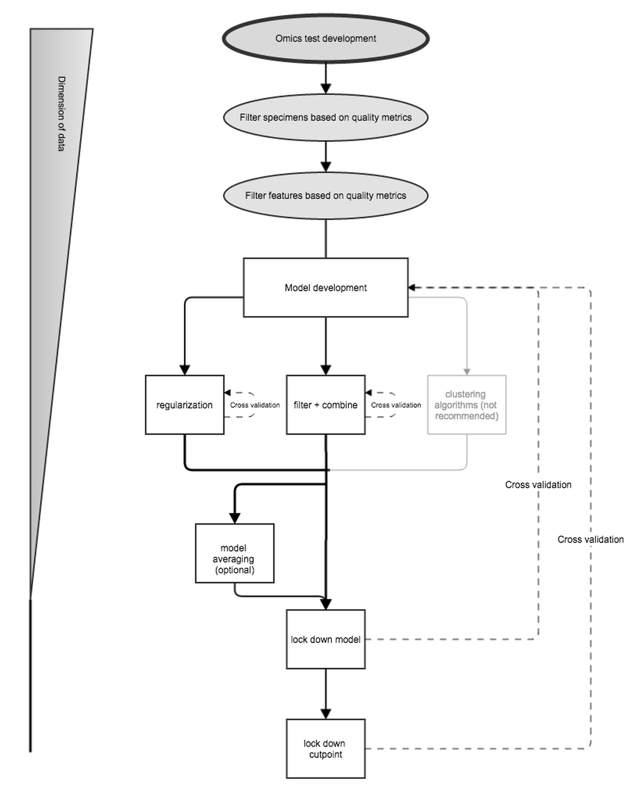
\includegraphics{figure1-2014-12-15.png}
\caption{Schematic illustrating the omics test development process.}
\end{figure}

\begin{figure}[htbp]
\centering
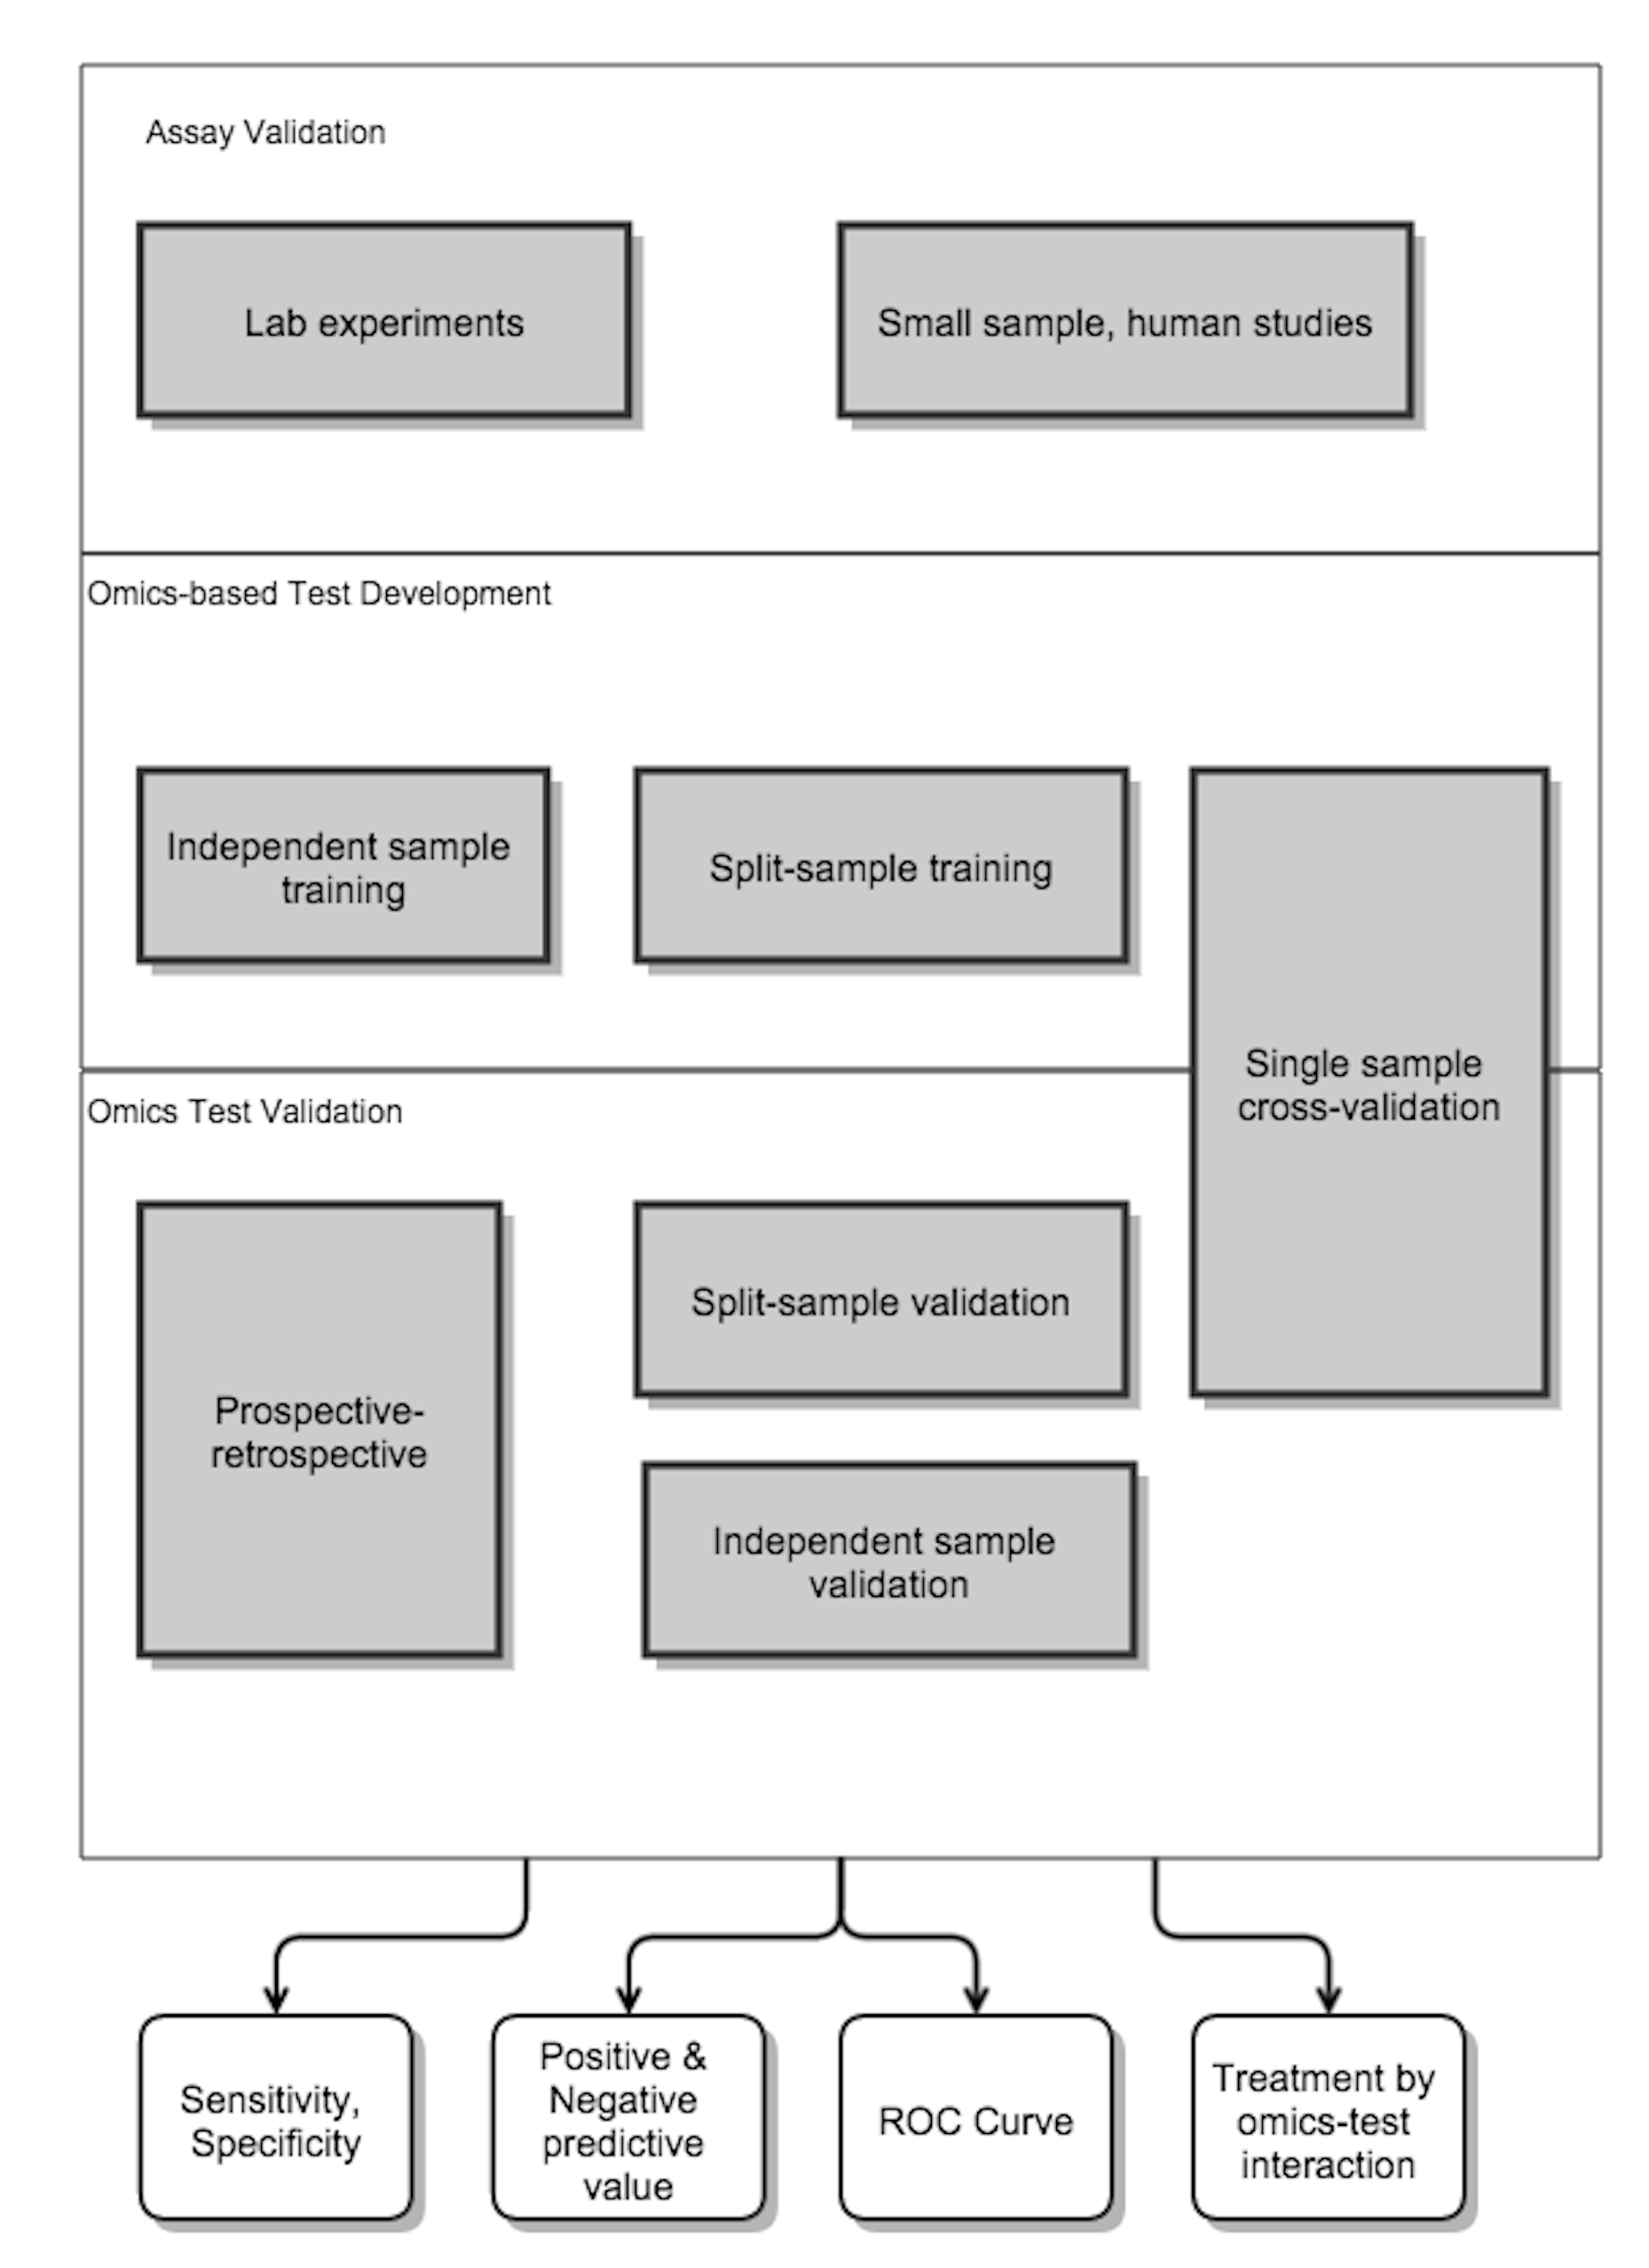
\includegraphics{figure2-2014-12-16.png}
\caption{Schematic illustrating the types of studies involved in omics
test assay validation, test development, and validation.}
\end{figure}

\section{Terminology}\label{terminology}

An omics-based test, or simply an \textbf{omics test}, is a mapping from
the set of features on the omics assay to a single number. This number
can be a binary value, such as good or poor prognosis, or it can provide
a continuous scale, such as a risk score. It must be feasible to perform
the test on an individual patient basis, by measuring the omics assay on
the individual's tissue. The assay generates a multitude of
measurements, which we will refer to as \textbf{features}, and then
fixed mathematical calculations are done to transform the many features
into the single test value. Examples of such features are gene
expression values, protein expression measurements, or genetic
mutations. We use the term \textbf{specimens} to refer to individual
patient tissues or fluids on which the assay would be run. We use the
term \textbf{sample} in the statistical sense, meaning a group of
individuals randomly selected from a population.

Investigators determine the way that the mathematical calculations are
done in the \textbf{development phase}. Often, there is a complete
sample which is randomly allocated into \textbf{development} and
\textbf{validation} sub-samples. These are also sometimes referred to as
\textbf{training} and \textbf{test} sets of samples. At the end of the
development phase, the model for the mathematical calculations is fixed
and the algorithm is locked down.

That model is evaluated definitively in the \textbf{validation} phase in
a completely independent sample. In order for the validation to be
unbiased and definitive, it is imperative that no information from the
validation sample leaks into the development phase. The validation
should mimic realistic clinical use as much as possible, and that means
that no further refinement to the test is allowed based on the observed
results.

A given study may cover only one of the many steps and the entire
process may be reported across multiple peer-reviewed publications. For
example, at least 4 key publications were devoted to the development and
validation of Oncotype DX, which is a commercially available omics-based
prognostic test used in breast cancer (4--7).

\section{What is the intended clinical
use?}\label{what-is-the-intended-clinical-use}

As with all clinical studies, the end goal is to improve patient care.
Omics studies are no different, and a clear statement of the intended
clinical use of the omics-test should be prominent. Carefully describing
the context for the use of the assay determines the type of study needed
to develop and validate it. The intended use of the assay also provides
an overarching context in which to interpret the population under study,
the assay measurements, and the statistical methods.

Omics-based tests in oncology generally are used for one of two clinical
purposes: prognosis or prediction of treatment response. A
\textbf{prognostic} test is used to predict the likely clinical outcome
of a patient. Often a prognosis is used to guide management of the
disease. Patients with a very good prognosis may opt not to receive any
treatment, while patients with a poor prognosis may opt for more
aggressive treatment. An omics-based prognostic test that is currently
used in practice is EndoPredict, which is used to predict the risk of
recurrence in ER-positive, HER2-negative breast cancer (8). For patients
with a low risk of recurrence, it has been demonstrated that the risks
of chemotherapy do not outweigh the benefits. Prognostic tests are
clinically useful for guiding general disease management.

\textbf{Predictive} tests are most useful for selecting patient
populations for treatment with specific targeted therapies. This
presumes the existence of a particular molecular targeted therapy. The
predictive test is used to identify patients who will benefit from the
targeted therapy. Predictive tests are generally based on only one or a
few molecular characteristics that the therapy targets. For example,
HER-2 is a gene that is associated with a more aggressive form of breast
cancer. Trastuzumab is a drug that specifically targets HER-2 and has
been shown to be effective in HER-2 positive breast cancer (9). While
targeted therapies generally target only one molecular characteristic,
omics assays can be used to identify molecular targets for less
well-understood drugs. However, most successful targeted therapies have
associated predictive tests that were developed based on the underlying
biology rather than a broad search over a large number of molecular
features (10).

\section{What is the patient population of
interest?}\label{what-is-the-patient-population-of-interest}

Along with the intended clinical use, a report should have a clear
statement of the intended population in which the test is being
evaluated. This could be broad or quite specific. For the omics test to
be useful, it must provide sufficient information above and beyond the
standard of care in the target patient population. The distribution of
the omics test and the expected benefit in the population should be
clearly specified in advance.

The expected benefit of a new omics-based test could differ greatly by
patient population. For instance, a prognostic test has more potential
for benefit in stage 2 breast cancer than it does in stage 1 breast
cancer, as the prognosis for stage 1 is already very good. Evaluating an
omics-based test in a broad populations that encompasses multiple stages
or multiple disease types can be difficult, as the test must provide
more information beyond that provided by standard clinical and
pathological factors.

\section{Are the assay methods and laboratory procedures
valid?}\label{are-the-assay-methods-and-laboratory-procedures-valid}

Analytical validation of an assay involves evaluating the performance of
the measurement in terms of accuracy, bias, and precision under a
variety of conditions. Conditions refer to pre-analytic factors such as
specimen quality, specimen collection, storage, and processing
procedures, and technical aspects such as laboratory technician and
batch effects from reagent lots or other assay materials. The
high-dimensional nature of omics data makes it very difficult to assess
each of the hundreds or thousands of outputs from a single assay. In
developing a omics-based signature that only uses a subset of the
components of a high-dimensional assay, one can analytically validate
the final signature alone. However, prior to developing the signature,
one must develop detailed standard operating procedures for specimen
handling and processing to ensure a baseline level of validity.

Study reports must state what type of specimens are used and whether the
test is applied to formalin-fixed paraffin embedded (FFPE) or only
fresh-frozen tissue. Most omics-based assays require a minimum
percentage of tumor to be successful. A report should clearly state what
criteria were used to screen tissue specimens prior to running the
assay. Generally this involves a criteria for the rejection of
poor-quality specimens on the basis of percent tumor, percent necrosis,
or some other marker of tissue quality.

Molecular assays can successfully be run on decades old FFPE tissue
(11). However, factors involved in the tissue processing and storage can
impact the analyte extraction and quality (12--14). Relatively little
attention has been given to studying the downstream effects of
pre-analytic factors on the individual omics features. In one study, the
authors observe that older FFPE specimens tended to have lower
expression levels and that this effect was different for different
genes. The investigators modified their assay to account for this
differential effect (15). Due to the high dimensionality of omics
assays, a small amount of bias on each feature can translate into large
errors when incorporating data from hundreds or thousands of features
into a single continuous measurement. Therefore it is important to
assess the impact of processing on the individual features in addition
to the overall test.

In addition to processing and storage, technical aspects of an assay can
impact the final results in a predictable way (16,17). There could be
technical effects, differences due to reagent lots, and other batch
effects. Such batch effects are commonly recognized yet often ignored in
high-dimensional assays (18). Efforts should be made to measure the
impact of these technical aspects and minimize them to the greatest
extent possible. The way in which specimens are assayed should be
randomized to prevent confounding batch effects with the clinical
outcome. Development and validation samples are sometimes run in the
same batch or with the same lot of technical aspects. This does minimize
batch effects, however, it can provide an overly optimistic assessment
of the test, because in clinical use, running specimens all in the same
batch is not always an option.

Similar to developing criteria for rejection of tissue specimens, in
omics settings, criteria should be developed for the rejection of
individual features (e.g.~genes, proteins) prior to the development of
the test, if problems cannot be resolved through improved assay
procedures. Features that do not pass the pre-specified quality metrics
should be removed from consideration from the final test. Note that this
feature processing step does not involve any clinical outcome
measurements. As a concrete example, in the development of the gene
expression based test EndoPredict, investigators chose to exclude probe
locations that have a dynamic range less than 2, probes for which fewer
than 1\% of the specimens had calls, and probes whose 90th percentile
was less than 350 units (8). Quality control steps of this nature can
ensure a more robust and reproducible development of the test.

Even with careful quality control and a locked down standard operating
procedure, it is difficult to completely eliminate the effects of
technical factors on assay results. Therefore, when designing the
development phase, the investigator must be mindful not to confound
technical factors with the clinical outcomes. The problem of batch
effects is widespread in omics research and can lead to spurious or
irreproducible results (18,19). As an extreme example, consider
developing an omics-based test to predict a binary clinical response. In
the development phase, all of the assays for the clinical responders
were run using reagent A, while all of the assays for the clinical
non-responders were run using reagent B. If it were the case that the
reagent has a significant effect on the assays, then the development
phase would then lead to what seems like an excellent predictor, except
it is predicting the batch effect rather than the clinical outcome.

\section{Are the statistical methods for test development
appropriate?}\label{are-the-statistical-methods-for-test-development-appropriate}

Once the analytical validity of the omics assay is established, the
features are translated into a binary classification, a multi-category
classification, or a continuous risk score. The methods used to perform
this translation must be carefully evaluated to ensure that the features
of the omics assay have been properly translated into a clinically
meaningful quantity.

Unfortunately, a common approach to developing prediction models is to
use cluster analysis of omics features, ignoring the clinical outcome
among the development samples. Cluster analysis is a class of methods
that is used to partition individuals into groups based on the
similarities or differences among the omics features (20). The number of
groups or clusters is not known in advance, but rather it is data
dependent. Clustering is unsupervised in the sense that discovery of the
groups is done without regard to the clinical outcome. The resulting
clusters are not designed to provide valid information regarding a
prognosis or prediction of response to therapy (21). A common argument
in favor of clustering is that it identifies biologically distinct
groups. However, the groups are identified using a statistical algorithm
and the biological relevance is only considered \emph{post hoc}. For
developing omics-based prognostic or predictive tests, it is better to
use supervised statistical methods which are designed to address those
aims, outlined below.

Often, there are more features measured than there are patients in the
sample. In such high-dimensional settings, it is required to identify a
subset of the features that will be used in the final multivariate
mathematical model. There are two broad statistical approaches to this
problem: \textbf{filtering} and \textbf{regularization}.

Filtering is a statistical approach where univariate methods are applied
to each of the many omics features in turn. Typically, the univariate
method involves estimating the association of the feature with the
clinical outcome. Then, a criterion, chosen in advance or selected using
cross-validation, is applied to the statistic to select a subset of
features. For example, suppose an investigator is interested in
developing a gene expression based test to predict clinical response to
a new therapy. For each of the 1000 gene expression features that are
available, one could compute a t-statistic comparing the expression
levels for responders versus non-responders. Genes with t-test p-values
greater than 0.0001 could be filtered out, and the remaining ones used
in a multivariable logistic regression model to predict response. (22)
describes a novel approach to filtering that is applied successfully to
predict B-cell lymphoma subtypes using gene expression microarrays.

Regularization is an approach in which all of the features in
consideration are entered into a special multivariable statistical model
for prediction of the clinical outcome, even if there are more features
than study participants. The special model includes a penalty component
which encourages the model to remove completely or downplay the impact
of features that are not relevant. There are various types of penalty
functions each with different properties, such as the lasso (23), the
ridge penalty (24), the elastic net (25), and others (20). Each type of
penalty term contains at least one tuning parameter, which may be
pre-specified or selected using cross-validation.

Each type of approach has its merits, and within each class there are a
variety of specific models to choose from. It is difficult to determine
what method will work best in advance. Instead of selecting a single
model to use, multiple models can be averaged to improve prediction
(26). This approach, called Bayesian model averaging, has proven
successful in different applications, including prediction of cancer
subtypes (27). It is more common, however, to try several different
methods then select the one that performs the best on a small subset of
the development sample. This is appropriate as long as the model
selection is done entirely separately from the final validation sample.
Leaking of information from the validation data into the model selection
process can cause bias in insidious ways.

In many oncology settings, such as pediatric cancers, patients and
specimens may be very sparse. It may be difficult to enroll sufficient
subjects to develop an omics test and then perform preliminary
validation on an independent sample. In that case, cross-validation can
provide an unbiased estimate of prediction error, if done properly (20).
Cross-validation refers to the idea that a model can be evaluated in the
same sample in which it is developed. Similar to a split sample
approach, in cross-validation only a small portion of the sample is left
out at a time. The model is estimated on the remaining samples, and the
performance is evaluated on the left out independent portion. This
process is repeated many times to get a more precise estimate of the
performance. (28) describe a cross validated trial design tailored for
sparse data settings.

In doing cross-validation, it is important to validate the entire model
estimation process, not only part of it. For that reason it is often
best to avoid complex test development procedures involving multiple,
data-driven selection steps and/or tuning parameters so as not to
mistakenly leak information from the validation data (29). More complex
procedures can also lead to overfitting, in which the model identifies
random noise in the data, rather than a true signal of clinical use.

\section{How is the validation study
designed?}\label{how-is-the-validation-study-designed}

Once the mathematical model is estimated and completely locked down
based on the development sample, a study to definitively evaluate the
locked-down test should be designed to address the clinical use in the
population of interest. The key characteristic of the evaluation study
or sample is that it is completely independent of the sample on which
the test was developed. Once the test is defined and locked down, no
information from the evaluation sample can be used to change the
features of the test. The evaluation sample could be a randomly selected
subgroup from the same parent study as the development set, or it could
be from a separate study altogether conducted in the same population. As
long as the population and the intended clinical use are clearly
defined, the evaluation can be done definitively.

A definitive evaluation can be done retrospectively, meaning that stored
specimens are selected from a study that has completed. The omics assay
is then run on the archived specimens and the locked down test is
associated with the clinical outcomes, which have already been observed
at the time of the assay measurement. This retrospective design can
yield high quality evidence of the test's characteristics, if it is done
carefully. It is imperative to develop a protocol for the study in which
the omics test is clearly and completely defined, the main hypotheses
are specified, and the assay standard operating procedures are detailed.
The archived specimens need to come from a study or trial with a
well-defined population under study, not a convenience sample. Sample
size and power calculations should be done with the same rigor as they
are in a clinical trial. Such a study, called
``prospective-retrospective'', can yield a high degree of evidence in
the evaluation of an omics-test, and with great efficiency. (30)

Alternatively, prospective studies can be used to evaluate an
omics-based test by performing the assay at the start of the study and
then following patients for clinical outcomes. Again, all of the key
details need to be specified up front in the protocol. The details of
the study design should be tailored to appropriately answer the clinical
question definitively. Several review articles are available that
describe the potential study designs for the evaluation of prognostic
and predictive tests (31--34). Details of specific designs and
statistical approaches are available for Bayesian approaches (35,36),
adaptive or sequential approaches (37,38), and standard frequentist
approaches (39--41). This has been and continues to be an active
research area in statistics, which means that designs are continually
evolving to appropriately address the clinical question in the
population of interest.

In the design, careful consideration should be given to the study power
and sample size. A prospective study in which patients may be undergoing
painful biopsies or unnecessary treatment should not be done unless
there is a high probability of definitively answering the scientific
question. Likewise, precious archived specimens should not be wasted on
a retrospective study that is under-powered. Most standard statistical
tools for power analysis apply to prognostic tests, however predictive
or therapy-guiding omics-based tests require a different approach. Many
protocols for predictive tests are powered to detect the interaction
effect between the treatment and the test (42). The existence of a
treatment-by-test-interaction is necessary but not sufficient for the
test to be useful in guiding therapy (43). Tools for power and sample
size analysis have been designed to specifically address the question of
a qualitative interaction (44--46).

\section{Are the development and validation samples strictly
separated?}\label{are-the-development-and-validation-samples-strictly-separated}

This issue has been discussed in previous sections, yet this error
occurs so frequently that it requires an in-depth discussion. The
evaluation sample for the assessment of a prognostic or predictive test
needs to be completely independent from the development sample. This is
especially true for omics-based tests, whose development is often
complex. Any information from the evaluation sample that leaks into the
development sample can bias the results, making tests appear better than
they truly are.

Leaking information between samples can happen in subtle ways.
Sometimes, part of the model development process is repeated on the
validation data. This is called partial resubstitution (21). For
example, a common model development approach is to first filter a subset
of 50 genes from a larger set of 450,000 based on their observed
association with the outcome. Then, the 50 genes are put into a
regression model to develop a single risk score. Occasionally,
investigators will perform the filtering on the development sample and
then re-estimate the regression model using the combined development and
validation samples. This gives overly optimistic estimates of the
performance of the algorithm. Partial resubstitution can be difficult to
detect when the model development is more complex, and if
cross-validation is used to estimate the performance.

In settings where relatively few samples are available, cross-validation
is an efficient and valid approach to estimating performance (47). The
key point whether using the split sample approach or cross validation is
that the entire model building process must be validated. Even informal
checks of the model on the validation sample, such as viewing survival
curve plots, prior to locking down the model can unknowingly cause bias.

\section{Are the statistical methods appropriate for test
validation?}\label{are-the-statistical-methods-appropriate-for-test-validation}

To assess the value of an omics-based test for prognosis or prediction
we need to estimate the association between the test and the clinical
outcome on an independent sample (the validation sample). Appropriate
statistics are essential to measure this association. Often,
investigators will report only the odds ratio (in the case of a binary
clinical outcome) or the hazard ratio (for a time-to-event clinical
outcome) for the omics test. The odds ratio or hazard ratio is
insufficient to determine the clinical utility of an omics-based test
(48). Ideally, a statistical method or set of statistical measures
should be chosen to address the intended clinical use of the test.

For a prognostic test, how often does the test correctly predict
recurrence (true positives) and how often does it correctly predict
non-recurrence (true negatives)? It is imperative to report both of
these measures, also known as the sensitivity and specificity, because
one can correctly predict all true positives simply by predicting that
all cases are positive. Is the performance good enough to change
clinical practice? Patients want to know the likelihood of recurrence
given their test results; this is called the positive predictive value.
If the likelihood of recurrence is very low overall in the population,
as it is in stage 1 breast cancer, then a new test must be highly
informative for it to be practice changing. For continuous-valued tests,
extensions to these measures exist and can be visualized with the
receiver operating characteristic (ROC) curve. Furthermore, extensions
also exist for time-to-event clinical outcomes such as overall or
progression free survival. (49) provides an excellent reference for
statistical measures for the evaluation of diagnostic and prognostic
tests.

In recent years, a number of potentially misleading statistical methods
have crept into common usage. The net reclassification index (NRI) and
its sibling, the integrated discrimination improvement (IDI), were
designed to assess the added value of a new test to existing criteria:
the incremental value. For example, it is often of interest to determine
whether a novel omics-based test adds value to standard clinical and
pathological features. The NRI and IDI specifically evaluate whether the
novel component enhances the differentiation of patients into risk
groups. This does not address the question whether the novel component
\emph{correctly} classifies patients (50,51). Others have noted
additional problems with the statistical operating characteristics of
the method, most importantly, that it is not a valid measure (52--54).
More fundamentally, it is not clear what clinical question this measure
addresses; does it matter if patients are classified differently if we
don't know whether they are classified correctly?

A proper evaluation of an omics-based test takes a comprehensive and
pre-specified approach to address the intended clinical use. For
predictive omics-based tests to guide therapy, a rigorous approach to
evaluation has been described, along with statistical software for
general use (55). This continues to be an active area of biostatistical
research.

\section{Concluding remarks}\label{concluding-remarks}

The use of omics-based tests for prognosis, predicting, and therapy
selection is steadily increasing in oncology. Careful evaluation of the
quality of studies by consumers of the clinical oncology literature is
imperative to provide a high level of patient care. Formal sets of
reporting criteria exist for the producers of such literature (1--3,56)
and these are also useful for readers to be aware of. We hope that the
discussion here has brought attention to the issues from the readers
perspective and will help promote critical evaluation of the relevant
literature.

\section{References}\label{references}

\setlength{\parindent}{0pt}

1. Altman DG, McShane LM, Sauerbrei W, Taube SE. Reporting
recommendations for tumor marker prognostic studies (rEMARK):
Explanation and elaboration. BMC Med 2012;10(1):51.

2. Janssens AC, Ioannidis J, Bedrosian S, et al. Strengthening the
reporting of genetic risk prediction studies (gRIPS): Explanation and
elaboration. Eur J Clin Invest 2011;41(9):1010--35.

3. McShane LM, Cavenagh MM, Lively TG, et al. Criteria for the use of
omics-based predictors in clinical trials: Explanation and elaboration.
BMC Med 2013;11(1):220.

4. Paik S, Shak S, Tang G, et al. A multigene assay to predict
recurrence of tamoxifen-treated, node-negative breast cancer. New
England Journal of Medicine 2004;351(27):2817--26.

5. Habel LA, Shak S, Jacobs MK, et al. A population-based study of tumor
gene expression and risk of breast cancer death among lymph
node-negative patients. Breast Cancer Res 2006;8(3):R25.

6. Cronin M, Sangli C, Liu M-L, et al. Analytical validation of the
oncotype dX genomic diagnostic test for recurrence prognosis and
therapeutic response prediction in node-negative, estrogen
receptor--positive breast cancer. Clin Chem 2007;53(6):1084--91.

7. Solin LJ, Gray R, Baehner FL, et al. A multigene expression assay to
predict local recurrence risk for ductal carcinoma in situ of the
breast. Journal of the National Cancer Institute 2013;105(10):701--10.

8. Filipits M, Rudas M, Jakesz R, et al. A new molecular predictor of
distant recurrence in eR-positive, hER2-negative breast cancer adds
independent information to conventional clinical risk factors. Clin
Cancer Res 2011;17(18):6012--20.

9. Fleeman N, Bagust A, Beale S, et al. Pertuzumab in combination with
trastuzumab and docetaxel for the treatment of hER2 positive metastatic
or locally recurrent unresectable breast cancer: A single technology
appraisal. 2013.

10. Sawyers CL. The cancer biomarker problem. Nature
2008;452(7187):548--52.

11. Iwamoto KS, Mizuno T, Ito T, et al. Feasibility of using decades-old
archival tissues in molecular oncology/epidemiology. The American
journal of pathology 1996;149(2):399--406.

12. Srinivasan M, Sedmak D, Jewell S. Effect of fixatives and tissue
processing on the content and integrity of nucleic acids. The American
journal of pathology 2002;161(6):1961--71.

13. Maldegem F van, Wit M de, Morsink F, Musler A, Weegenaar J, Noesel
CJ van. Effects of processing delay, formalin fixation, and
immunohistochemistry on rNA recovery from formalin-fixed
paraffin-embedded tissue sections. Diagn Mol Pathol 2008;17(1):51--8.

14. Specht K, Richter T, M{ü}ller U, Walch A, Werner M, H{ö}fler H.
Quantitative gene expression analysis in microdissected archival
formalin-fixed and paraffin-embedded tumor tissue. The American journal
of pathology 2001;158(2):419--29.

15. Cronin M, Pho M, Dutta D, et al. Measurement of gene expression in
archival paraffin-embedded tissues: Development and performance of a
92-gene reverse transcriptase-polymerase chain reaction assay. The
American journal of pathology 2004;164(1):35--42.

16. Pennello GA. Analytical and clinical evaluation of biomarkers
assays: When are biomarkers ready for prime time? Clin Trials
2013;10(5):653--65.

17. Isler JA, Vesterqvist OE, Burczynski ME. Analytical validation of
genotyping assays in the biomarker laboratory. Pharmacogenomics
2007;8(4):339--52.

18. Leek JT, Scharpf RB, Bravo HC, et al. Tackling the widespread and
critical impact of batch effects in high-throughput data. Nat Rev Genet
2010;11(10):733--9.

19. Soneson C, Gerster S, Delorenzi M. Batch effect confounding leads to
strong bias in performance estimates obtained by cross-validation. PloS
one 2014;9(6):e100335.

20. Hastie T, Friedman J, Tibshirani R. The elements of statistical
learning. Springer; 2009.

21. Simon R, Radmacher MD, Dobbin K, McShane LM. Pitfalls in the use of
dNA microarray data for diagnostic and prognostic classification. J Natl
Cancer Inst 2003;95(1):14--8.

22. Bair E, Tibshirani R. Semi-supervised methods to predict patient
survival from gene expression data. PLoS Biol 2004;2(4):e108.

23. Tibshirani R. Regression shrinkage and selection via the lasso.
Journal of the Royal Statistical Society Series B (Methodological)
1996;58(1):267--88.

24. Hoerl AE, Kennard RW. Ridge regression: Biased estimation for
nonorthogonal problems. Technometrics 1970;12(1):55--67.

25. Zou H, Hastie T. Regularization and variable selection via the
elastic net. Journal of the Royal Statistical Society: Series B
(Statistical Methodology) 2005;67(2):301--20.

26. Hoeting JA, Madigan D, Raftery AE, Volinsky CT. Bayesian model
averaging: A tutorial. Statistical science 1999;14(4):382--401.

27. Yeung KY, Bumgarner RE, Raftery AE. Bayesian model averaging:
Development of an improved multi-class, gene selection and
classification tool for microarray data. Bioinformatics
2005;21(10):2394--402.

28. Freidlin B, Jiang W, Simon R. The cross-validated adaptive signature
design. Clin Cancer Res 2010;16(2):691--8.

29. McShane LM, Polley M-YC. Development of omics-based clinical tests
for prognosis and therapy selection: The challenge of achieving
statistical robustness and clinical utility. Clin Trials
2013;10(5):653--65.

30. Simon RM, Paik S, Hayes DF. Use of archived specimens in evaluation
of prognostic and predictive biomarkers. J Natl Cancer Inst
2009;101(21):1446--52.

31. Sargent DJ, Conley BA, Allegra C, Collette L. Clinical trial designs
for predictive marker validation in cancer treatment trials. Journal of
Clinical Oncology 2005;23(9):2020--7.

32. Baker SG, Kramer BS, Sargent DJ, Bonetti M. Biomarkers, subgroup
evaluation, and clinical trial design. Discov Med 2012;13(70):187--92.

33. Freidlin B, Korn EL. Biomarker enrichment strategies: Matching trial
design to biomarker credentials. Nature Reviews Clinical Oncology
2014;11(2):81--90.

34. Mandrekar SJ, Sargent DJ. Clinical trial designs for predictive
biomarker validation: Theoretical considerations and practical
challenges. J Clin Oncol 2009;27(24):4027--34.

35. Brannath W, Zuber E, Branson M, et al. Confirmatory adaptive designs
with bayesian decision tools for a targeted therapy in oncology. Stat
Med 2009;28(10):1445--63.

36. Morita S, Yamamoto H, Sugitani Y. Biomarker-based bayesian
randomized phase iI clinical trial design to identify a sensitive
patient subpopulation. Stat Med 2014;33(23):4008--16.

37. Freidlin B, Korn EL, Gray R. Marker sequential test (maST) design.
Clin Trials 2014;11(1):19--27.

38. Jiang W, Freidlin B, Simon R. Biomarker-adaptive threshold design: A
procedure for evaluating treatment with possible biomarker-defined
subset effect. J Natl Cancer Inst 2007;99(13):1036--43.

39. Denne JS, Pennello G, Zhao L, Chang S-C, Althouse S. Identifying a
subpopulation for a tailored therapy: Bridging clinical efficacy from a
laboratory-developed assay to a validated in vitro diagnostic test kit.
Statistics in Biopharmaceutical Research 2014;6(1):78--88.

40. Eng KH. Randomized reverse marker strategy design for prospective
biomarker validation. Stat Med 2014;33(18):3089--99.

41. Freidlin B, McShane LM, Polley M-YC, Korn EL. Randomized phase iI
trial designs with biomarkers. J Clin Oncol 2012;30(26):3304--9.

42. Peterson B, George SL. Sample size requirements and length of study
for testing interaction in a 1 x k factorial design when time-to-failure
is the outcome. Control Clin Trials 1993;14(6):511--22.

43. Polley M-YC, Freidlin B, Korn EL, Conley BA, Abrams JS, McShane LM.
Statistical and practical considerations for clinical evaluation of
predictive biomarkers. J Natl Cancer Inst 2013;105(22):1677--83.

44. Gail M, Simon R. Testing for qualitative interactions between
treatment effects and patient subsets. Biometrics 1985;41:361--72.

45. Bayman EÖ, Chaloner K, Cowles MK. Detecting qualitative interaction:
A bayesian approach. Stat Med 2010;29(4):455--63.

46. Mackey HM, Bengtsson T. Sample size and threshold estimation for
clinical trials with predictive biomarkers. Contemp Clin Trials
2013;36(2):664--72.

47. Lee S. Mistakes in validating the accuracy of a prediction
classifier in high-dimensional butsmall-sample microarray data. Stat
Methods Med Res 2008;17(6):635--42.

48. Pepe MS, Janes H, Longton G, Leisenring W, Newcomb P. Limitations of
the odds ratio in gauging the performance of a diagnostic, prognostic,
or screening marker. Am J Epidemiol 2004;159(9):882--90.

49. Pepe MS. The statistical evaluation of medical tests for
classification and prediction. Oxford University Press; 2003.

50. Hilden J, Gerds TA. A note on the evaluation of novel biomarkers: Do
not rely on integrated discrimination improvement and net
reclassification index. Stat Med 2013;33(19):3405--14.

51. Pepe MS. Problems with risk reclassification methods for evaluating
prediction models. Am J Epidemiol 2011;173(11):1327--35.

52. Pepe MS, Janes H, Li CI. Net risk reclassification p values: Valid
or misleading? J Natl Cancer Inst 2014;106(4):doi:10.1093/jnci/dju041.

53. Kerr KF, Wang Z, Janes H, McClelland RL, Psaty BM, Pepe MS. Net
reclassification indices for evaluating risk prediction instruments: A
critical review. Epidemiology 2014;25(1):114--21.

54. Hilden J. Commentary: On nRI, iDI, and “Good-looking” statistics
with nothing underneath. Epidemiology 2014;25(2):265--7.

55. Janes H, Brown MD, Huang Y, Pepe MS. An approach to evaluating and
comparing biomarkers for patient treatment selection. The international
journal of biostatistics 2014;10(1):99--121.

56. Bouwmeester W, Zuithoff NP, Mallett S, et al. Reporting and methods
in clinical prediction research: A systematic review. PLoS Med
2012;9(5):e1001221.

\end{document}